	\section{Introduction}
%
%1. Context
%2. Problem
%3. Problem relevant and nontrivial
%4. Not solved before
%5. My Plan for solving it

``To move at full speed, it’s crucial to bring the networking operations teams into the DevOps chain...''\footnote{https://siliconangle.com/2019/02/19/cloud-native-networking-for-devops-leaves-sdn-in-the-dust-cubeconversations-startupoftheweek/}.

Many advances have been made in recent years towards making applications ready for the special environment of the cloud. The development procedure for these type of programs needs to be adapted in order to be effective and efficient since it significantly departs from previous settings. Matthew Foemmel and Martin Fowler have proposed the influential practice of continuous integration and deployment \cite{fowler_2006} \cite{fowler_foemmel_2000} in order to tackle the development side of this complex process. In their original work from 2000 they base their approach on four principles: A single place for the source code shall be used, the build and test process needs to be automated and the resulting executable artifact has to be reachable.
The process provides a solid basis for the collaboration on any software project, but is especially useful when working on a project that has its place in the cloud. 

This paradigm has been expanded to not only comprise the development part, but also architectural best practices in the so-called 12-factor methodology as formulated by Adam Wiggins and drafted by employees of the cloud platform Heroku. It summarizes the most important aspects that need to be taken into consideration to make life easier when designing cloud native applications. These guidelines contain strategies to avoid recurring problems when developing in the cloud environment, like the fragmentation of the codebase, keeping track of and managing all needed dependencies, placing the configuration in the environment and many more \cite{hofmann2017microservices} \cite{12Factor}. 

While there have been many advances in making applications ready for the cloud  and using automated build chains like in Continuous Integration and Delivery, the networking infrastructure has long remained old-school monolithic and thus costly to acquire and maintain, a situation that discourages innovation and has long been known as \textit{internet ossification} \cite{nunes2014survey}. Functionalities that are specific to the setup, orchestration, administration and enhancement of large scale networks have long been implemented inside specialized hardware middleboxes. Such services range from the security domain (intrusion detection, firewalls) to the optimization of the Wide Area Network (WAN). Deploying and managing dedicated hardware in this scenario quickly results in high investment as well as operation costs and hugely limits the flexibility of the network. With the ever growing reliance on cloud networks and infrastructures to provide a plethora of services, it is crucial to make the management of the underlying network much more reactive and adaptable. 

In order to take full advantage of the highly modular and flexible cloud concepts, the supporting network has to be able to quickly and reliably adapt to changes. The guiding question for this paper is to \textit{give an overview and evaluate concepts that have been put forward to tackle these limitations by applying the cloud native principles to the network domain.}

Before focusing on the virtualization of specific network functions, the concept of Software Defined Networks will be introduced as a related and very powerful and promising technology. Under this paradigm, the network hardware like the switches orchestrating the data and packet flow, will need to provide means for external configuration. This reorganization is absolutely necessary to break up these highly integrated devices that do not allow for a central and automatic configuration. After having achieved means to externalize the ability to modify and control their behavior via a centralized software controller, all switching hardware can be configured at once from one location. This facilitates the deployment and enforcement of policies and makes the network \textit{programmable}. This programmability is key to quickly provisioning and integrating new instances of network components. 

A first step towards easier deployment of network functionality can be taken by providing network functions  and services that have traditionally been dependent on proprietary and custom hardware as \textit{virtualized and independent software entities} that can run on general-purpose hardware. This should break up the dependency on specialized middleboxes, and facilitate the provisioning and management of the services. Although virtualization has had a great impact, there still are unsolved problems that need addressing. These include and are not limited to the speed of upgrades and restarts, restricted scalability and the fact that often services have been ported to the cloud in a \textit{lift and shift manner} without taking full advantage of the cloud paradigm \cite{CNF}.

In a second step it is important to find solutions to these problems, especially when thinking about how it is possible to efficiently design and manage virtualized network functions. Orienting them along the lines of the cloud has coined the term of \textit{Cloud Native Network Functions} \cite{CNF} \cite{cn5gvnf} \cite{evolutionnfv}. 

\section{Related Work}
The Cloud-native Network function is a young field of research that continues the trend from breaking up rigidity in large scale networks. Consequently, few works exist capturing the essence of the new Cloud-native paradigm in the network domain.

Imadali \textit{et al.} have given a short insight into the design principles that need to be taken into account when defining Cloud-native Network Functions. Following that, they provide insight into existing NFV projects and discuss a new cloud service model, namely \textit{5G as a Service} that could for instance be used in a scenario where Radio Access Networks are being deployed and shared among multiple tenants. Following that, they defined a \textit{5G CN-VNF} framework, used to make networking infrastructure accessible. By no means is this production ready, but provides a good introduction to the subject and shows how tools to ease development in this regards can be designed \cite{cn5gvnf}.

A whitepaper by the 5G-PPP titled \textit{From Webscale to Telco, the Cloud Native Journey} \cite{5gppp} emphasizes the relevance of this new computing paradigm especially for the telecommunications industry. The structure of the work shows what the main enablers are for implementing and realize the new use and business cases of fifth generation networks. Software architecture principles as defined in the twelve factor app and the microservice architecture are among them, as well as open source software following useful standards.

Finally, Telco and networking providers also postulate their views on CNFs especially in the context of 5G. Among the companies that have authored such a paper are Cisco \cite{CNF}, Huawei \cite{evolutionnfv}, Ericsson \cite{ericsson} and many more. Financial interests often lie behind this kind of publication from enterprises, which can be a double-edged sword: On the one hand, the motivation might be to promote services and devices to drive sales. On the other hand, this provides an interesting insight into which technologies are deemed possibly realizable and profitable.
\section{Physical Network Service Composition}
\label{sec:physical}
Before venturing into Virtualized Network Functions, it needs to be clarified what network functions are in general, how they are implemented and composed \textit{physically}, and what the motivations are to move towards virtualizing them. 

Networks are the backbone of any modern IT infrastructure, and with the unstoppable rise of  Cloud Computing services their importance is ever increasing. This sharp rise in relevance causes the setup and operation of previously unthinkable data centers. Providing specific functioniality in such an environment has traditionally been the task of dedicated hardware that implemented services of many different domains. These include security functions that setup firewalls, scan for viruses and detect intruders but might be applied to ``...to any data plane packet processing and control plane function...''\cite{nfv_wp}. The advantage of using Application-specific integrated circuit (ASICs) lies in the potential for optimization. When designing a device that serves a very specific purpose, the application scenario can be anticipated much better than with general-purpose hardware. This typically leads to lower power consumption, higher efficiency and better output, but drives up the purchasing cost. Additionally, the operational cost is also high, since acquiring, configuring, deploying and maintaining such middleboxes is often a tedious, manual-heavy task. Nevertheless, this type of \textit{physical} function delivery has historically been the primary way of building and operating networks, especially in a data center or telecommunication and internet service provider environment. This is due to the fact that there have not been production-ready, open source solutions available that could have been deployed on so-called \textit{whiteboxes}. White boxes are devices built from general-purpose hardware that are often employed in software defined networks, due to their modifiable nature. The logic was rather already integrated in the hardware, with almost no chance of customizing them.


\begin{figure}[h]
	\centering
	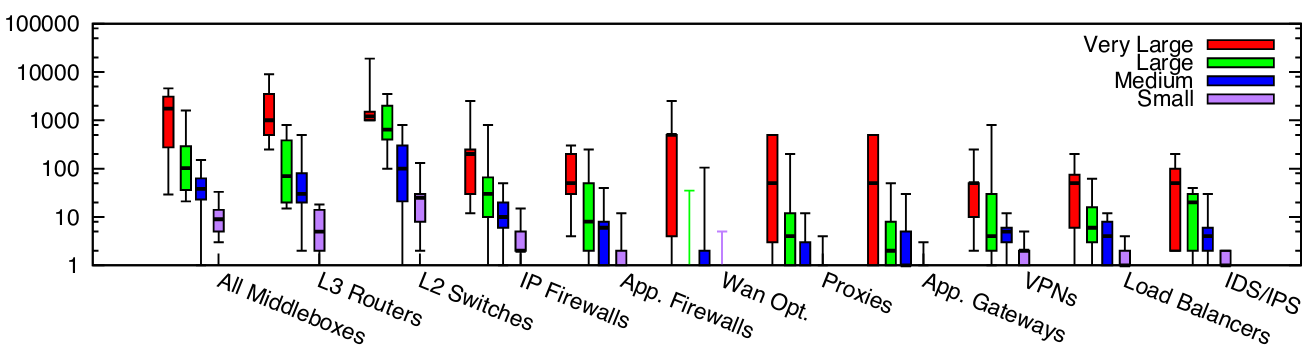
\includegraphics[width=1\linewidth]{images/middleboxesNumbers.png}
	\caption{Middlebox deployments in enterprise networks of various size (< 1k - >100k hosts). Y-axis in log scale, source \cite{sherry2016middleboxes}}
	\label{img:middleboxesNumbers}
\end{figure}

\begin{figure}[h]
	\centering
	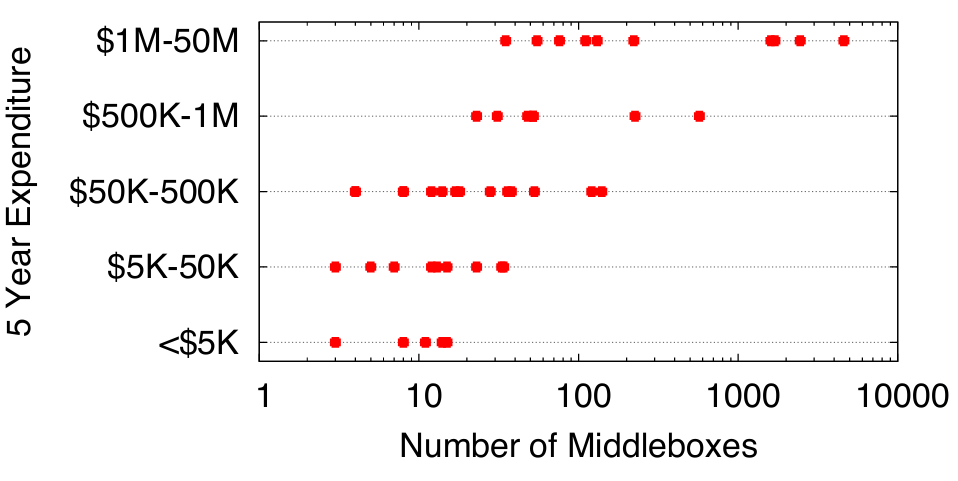
\includegraphics[width=1\linewidth]{images/middleboxesCost.png}
	\caption{Administrator-estimated spending on middlebox hardware per network \cite{sherry2016middleboxes}}
	\label{img:middleboxesCost}
\end{figure}

Figure \ref{img:middleboxesNumbers} illustrates the sheer amount of devices that are needed to guarantee the operation of enterprise networks of various size. Sherry \cite{sherry2012survey} \cite{sherry2016middleboxes} investigated their distribution among 57 educational and enterprise networks by surveying the operators for their experiences with the network appliances. Special focus was put on the quantity, their concerns, the cost and the ease of management. The results of this work give a good indication why this situation is unsustainable for future networks:  The number of these boxes is very high. To put it into perspective, the amount of these function specific devices approaches that of fundamental hardware like L3/L2 infrastructure. The associated cost of deploying such a large number of devices can be inspected in figure \ref{img:middleboxesCost} and indicates that investment cost is skyrocketing. Naturally, this might not be a problem for small companies that use a little amount of these devices. However, Cloud and Internet Service Providers rely on building, maintaining and reorganizing enormous computer networks and thus are driving forces behind alternative concepts in this domain \cite{sherry2016middleboxes} \cite{sherry2012survey}.


\section{Network Virtualization}
This will only gain importance with higher complexity and higher demand of the networks that are being built. Growing cloud data centers, implementation of 5G, further demanding services provided in the cloud like for instance Google Stadia, a streaming service for gaming. The last one is a very interesting scenario since low latency and high bandwidth is of utmost importance and needs to be guaranteed. \todo{source} Additionally, the provisioning and deployment of resources needs to happen instantly. This project might be paving the way for more ``serious'' applications like taking over functionality in autonomous driving. 

Another relevant use case scenario includes the possibility of implementing a \textit{tactile internet} that allows to put distant environments in someone's reach. Such a scenario where this might be needed is remote surgery, where a surgeon would use a remote controlled robot to perform a procedure in a distant place. In order for this to work, unforeseen latency, fault-tolerance and reliability has to be ensured. Fulfilling such demanding requirements is only possible if the supporting network is highly flexible and can guarantee not only continuous connectivity, but also high performance. 

The previously described problem can only be solved when the need for the manual configuration and deployment that takes place on a box-to-box basis of function-specific hardware can be eliminated. The answer to this challenge is virtualization of the functionality in question which makes it both more configurable and highly maintainable. In order to take advantage of this virtualization, though, the encompassing network needs to support feasible possibilities to manage the virtual instances of network functions. Without a degree of automation and a centralized, programmatic approach, there would not be a huge benefit of going from physical to virtual. Software Defined Networking is ideal and often goes hand in hand with using these cutting edge technologies.

Aside from the performance standpoint, this is also an ideal way to reduce cost significantly. This is due to multiple factors, such as the high purchasing cost of the middleboxes. Additionally, the devices often provide vendor-specific means for configuration which entails high administrative and operational cost since personnel training and special spare parts are needed.  The investment into retraining the staff that has to work with such devices can even influence the decision making process since without the expertise, smooth operations of the network are questionable. 

Once it is time to update or upgrade the parts of the network that provide certain functionality, another advantage becomes quickly apparent: With purpose-specific hardware, the only way to to get the newest features is to replace the outdated hardware with the newer model. And if more instances of the functionality is needed, there acquiring more devices is the only choice to allow for scalability or provide fault tolerance via replication. Additionally, when a new appliance comes out, until it has been successfully deployed, it often already is outdated. With softwarized instances of this functionality, proven software development practices can easily be applied in order to mitigate this problem. Updates, upgrades or in the worst case, reinstallation of a program guarantee an easy path to deploy the newest functionality. Replication of a service can also be done much easier and quicker by means of virtualization. Spinning up an additional virtual machine, or in later scenarios another container, is more practical than relying upon physical boxes. 

As already mentioned, virtualization and providing the network functionality as software packages that can run on general-purpose hardware anywhere is the core promise of network virtualization. This principle has caused a paradigm shift in recent years in networking that has lead to many projects and software solutions. In the following sections Software Defined Networking (SDN), Network Function Virtualization (NFV) and Virtualized Network Functions (VNF) will be briefly introduced as the main driving forces and central ideas behind the virtualization efforts. 


\subsection{Software Defined Networking}
\label{sec:sdn}

The unobstructed operation of highly distributed applications and the offer of services depends highly on mitigating faults in the network and the appropriate reaction to fluctuating load. In traditional networks, there is hardly any support to implement automatic policy change as a reaction to events like spikes in load or the reconfiguration when faults occur in the system \cite{kreutz2015software}. When faced with such situations, ''[\dots] every single hardware instance [\dots]`` \cite{grossmann2013auto} is in need for manipulation to realize the desired change.  The need for manual intervention is responsible for immense risk regarding service interruption. The high complexity associated with this kind of networks introduces a lot of inertia and in the worst case ends in a state known as \textit{ossification} \cite{nunes2014survey}. Providing network abstractions as a service is unthinkable in such a scenario, since quick, automatic and seamless planning, provisioning and reliable configuration can not be guaranteed.

\begin{figure}[h]
	\centering
	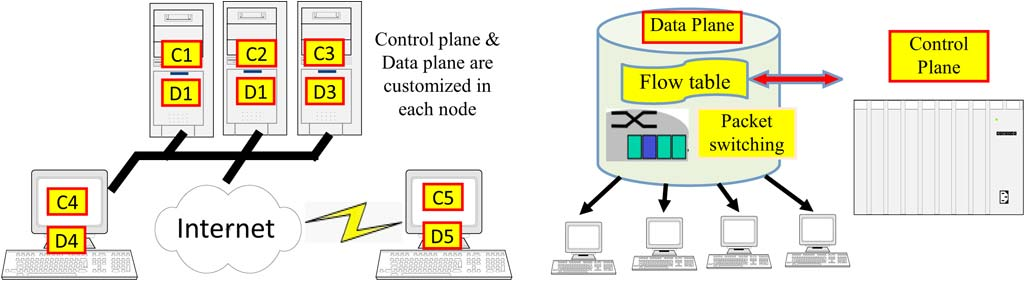
\includegraphics[width=0.48\textwidth]{images/sdn.png}
	\caption{Comparison between traditional (left) and Software-defined Networks (right), source \cite{li2015software}}
	\label{img:sdn}
\end{figure}
%PNF to NFV
Breaking up the rigidity is of utmost importance to building more flexible and cheaper networks that can  meet the demands of the future. Software Defined Networking is the technology of choice when there is a need for programmable networks. The core premise is the separation of the so-called control- and data planes, which are traditionally vertically integrated in switching devices. The logic that controls the packet forwarding and orchestration of the data flow is located inside the devices, just as well as the data structure that stores the rules for forwarding. This disallows for external manipulation while introducing the need for relying upon the vendor spefic way of configuration and thus ''[\dots]  reducing flexibility and hindering innovation [\dots]``\cite{kreutz2015software}.

In SDN the control layer is being externalized and abstracted from all the switching infrastructure into an external controller instance that provides multiple means of organizing and configuring the traffic flow in the managed devices. Figure \ref{img:sdn} provides a comparison between the two concepts, where the traditional, vertically integrated switches can be seen on the left. Each device contains its own logic that controls the incoming and outgoing packets. Additionally, a middlebox that might provide the functionality of a firewall, is closely attached to the middlebox on the right circumventing the problem that the switches and routers only provide limited configuration. Problems arising from the reliance on such middleboxes have been discussed in section \ref{sec:physical}.  On the right hand side, the control plane has been externalized from the three nodes into a centralized software control. The solid edges represent data flow, while the dashed lines show the control and monitoring traffic that takes place between the controller and the boxes under its domain.

\begin{figure}[h]
	\centering
	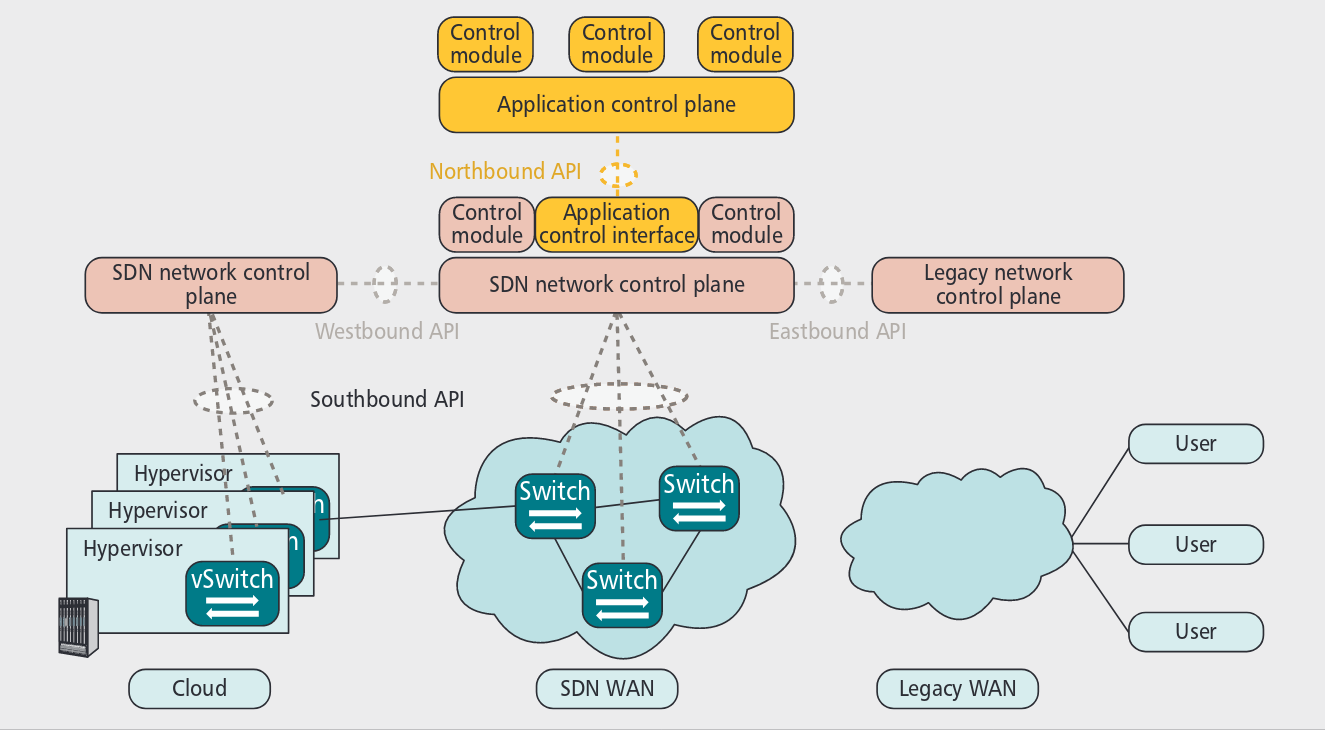
\includegraphics[width=0.49\textwidth]{images/sdnAPIs.png}
	\caption{The different elements of the SDN architecture, connected via several APIs. The northbound for application communication, westbound for inter controller synchronization, eastbound for legacy networks and southbound for device communication, source \cite{jarschel2014interfaces}}
	\label{img:sdnAPIs}
\end{figure}

In this kind of architecture, there are multiple, very important advantages: Policies can be defined and enforced on all devices almost instantly, without the need for cumbersome, vendor-specific configuration effort. The boxes no longer need to implement any control logic, and are reduced to forwarding switches that only need to support the communication with an SDN controller. Visualization and monitoring of the devices is taken care of by the same program, facilitating the operation and problem solving. A common protocol provides the basis for communication and the sending of commands between the devices and the controller that can run on any kind of hardware. Finally, such controllers often provide an API to write custom applications, allowing for very fine-grained customization that circumvents the need to wait for a hardware vendor to implement and roll-out a new feature. As a side note, since this figure suggests the controller constitutes a single point-of-failure, many controllers support the concept of clustering. Deploying multiple instances mitigates the risks when one is failing. 

Programming of the devices throughout the network works over a standardized protocol that allows to manipulate the data or forwarding plane of each device. The Open Network Foundation (ONF) develops and manages \textit{OpenFlow}, a protocol that was originally proposed so that researchers could ''[\dots] run experiments on heterogeneous switches in a uniform way at line-rate and with high port-density;``\cite{mckeown2008openflow}. As the technology matured, it has become one of the best known enabling technology for SDN. Generally speaking, a software controller can support multiple of these protocols via its Southbound API making it even more flexible. The choice of such a protocol depends on what protocols the managed devices support mainly. 

With OpenFlow for instance, a controller can manipulate a so-called \textit{flow table } for each switch. This table represents the packet forwarding rules that determine the handling of an incoming packet. If no rule applies, the standard behavior is to send the packet for further analysis to the controller, which will then analyze the packet. This is where the power of SDN comes to play, since an in-depth analysis of the packet can reveal useful information that can be used to determine how to deal with it. The packet can be ignored, it can be forwarded and new rules and routes can be established, or a custom application could trigger an alarm or even trigger the deployment of a new service that might be overloaded or missing. Extending the logic via additional applications is done via the Northbound API. The Westbound API is needed to provide the communication between multiple instance of the controller software. These might be needed to provide fault tolerance or a logical separation of the devices. The last API is located Eastbound and provides a point of communication with legacy networks and downward compatibility. All these different elements that make up an SDN controller can be inspected in Figure \ref{img:sdnAPIs}.

East and Westbound APIs are not part of all architecture specifications and present in Sezer \textit{et al.} \cite{sezer2013we} for instance. The authors reserve the west- and eastbound APIs for inter cluster communication of multiple controller instances. \cite{hu2014survey} \cite{jarschel2014interfaces} \cite{nunes2014survey} \cite{sezer2013we} \cite{shin2012software} \cite{jammal2014software}.

\subsection{NFV}
\begin{comment}
 \begin{description}
 	\item often monolithic, scaling coarse grained, whole vnf needs to be replicated
 	\item some functions repeatedly (unnecessarily) called in sercice function chains
 	\item vnf as a bumb in the wire
 	\item \cite{chowdhury2019re}
 \end{description}
\end{comment}

\subsubsection{NFV SDN relationship}
% NFV SDN relationship
Putting a controller in charge of the switching infrastructure in a network allows for flexibility and network programmability. This concept is complementary to that of providing functions in a virtualized manner that have previously been running on purpose-specific hardware. These two concepts do not necessitate each other, since they can be deployed and used independently. Nevertheless, they are in support of the same idea: Facilitating the network setup, operation and upgrade via the means of virtualization and softwarization. Their relationship is so close even that the white paper for NFVs dedicates a subsection to this. Making use of both concepts can proof mutually beneficent since ''[\dots] approaches relying on the separation of the control and data forwarding planes as proposed by SDN can enhance performance, simplify compatibility with existing deployments, and facilitate operation and maintenance procedures. Network Functions Virtualization is able to support SDN by providing the infrastructure upon which the SDN software can run`` \cite{nfv_wp}. 


% NFVs 
\subsubsection{PNF to VNF}
After SDN has introduced a paradigm which promises flexible reconfiguration of a network, the idea of running network functions on general purpose hardware in virtualized environments in the form of \textit{NFV} has taken shape. Leaving behing ASIC boxes and orienting oneself towards software solutions lie at the heart of this technique. ETSI, the European Telecommunications Standards Institute, comprised by multiple telecommunications providers and operators, has put forward a white paper in 2012 defining critical aspects in 2012 \cite{nfv_wp}. After this had been published, this proposal has gained a lot of momentum and implementations that allow to make use of this new technology have been put forward, which are taken into consideration when planning and building networks \cite{ordonez2017network}.

\begin{figure}[H]
	\centering
	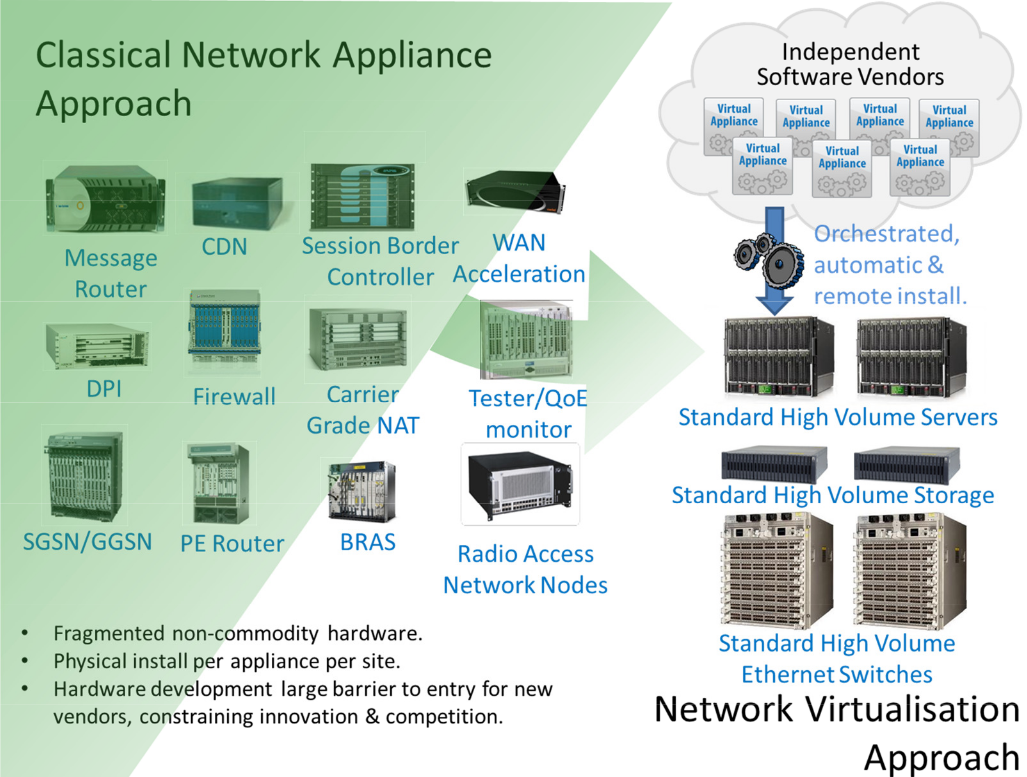
\includegraphics[width=0.5\textwidth]{images/nfv.png}
	\caption{From ASICs, to virtual appliances, source \cite{nfv_wp}}
	\label{img:nfv_wp}
\end{figure}

Figure \ref{img:nfv_wp} visualizes why SDN and NFV are often described as a \textit{paradigm shift}. The network landscape and physical composition can change considerably as the shift from left to right indicates. The left side shows the classical approach, relying on a multitude of heterogeneous, vendor-specific and non-standardized devices that are built for one specific purpose. These \textit{black boxes} are scattered all over and need to be manually configured in order to work. Implementing their functionality in pure software packaging it into artifacts that can be executed on standard devices present throughout the network, provides an unprecedented liberty in composing and orchestrating the functionalities present in a network. Decoupling the actual application logic from their physical surroundings also favors the emergence of a broader ecosystem where such programs are developed and shared, rendering this concept even more appealing.

\subsubsection{NFV Architecture}
Virtual appliances can either be developed or procured from emerging software ecosystems. As a part of this vision, an orchestrator platform should take care of automatic procedures like fetching and installing it onto appliances present in the network. The configuration for the packet flow then can be done via SDN (not part of the figure) which shows why these two concepts go hand in hand. 

A conceptual architecture overview is given in Figure \ref{img:nfv_ref_arch}, where several layers are combined to build a reliable and functional system. The bottom summarizes the physical hardware resources available providing different basic functionalities like \textit{compute, storage} and \textit{network}.  By exploiting the available infrastructure, a virtualization layer provides an abstraction that can be used to easier define and provide access to a required set of resources and schedule their provisioning. Predefined and runnable VNFs can subsequently be executed on the abstracted virtualized compute, storage and network devices. The systems that have been built in recent years often use virtual machines to bundle the functionality inside an artifact that can be executed almost anywhere. In order to fulfill the vision of network function virtualization and realize its full potential, automation is key. This is part of the NFV orchestrator's job, that can be fed service deployment requirements and thus reserve the resources needed and deploy the function.

\begin{figure}[H]
	\centering
	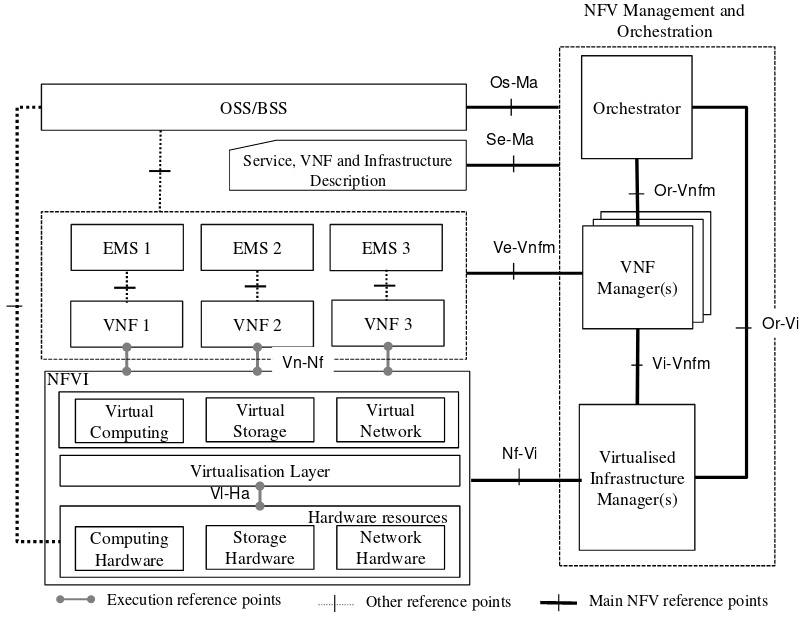
\includegraphics[width=1\linewidth]{images/nfv_ref_arch.png}
	\caption{Reference NFV architecture \cite{etsi1etsi}}
	\label{img:nfv_ref_arch}
\end{figure}

In order to ensure that virtual machines are started and stopped as needed, so that there is a platform for the VNFs to run on, there is another entity needed, namely the Virtualized Infrastructure Manager (VIM). Its responsibilities are focused on mapping the resource needs of the VNFs to specific VMs. The manager has therefore to be in charge of the underlying software that can realize such an infrastructure, including for instance hypervisors, and also the resources needed such as compute, storage and network. Allacating resources for function deployment falls also under its domain by by instantiating virtual machines onto hypervisors. After the initial setup, it should take care of allocating additional resources to VMs and further optimizing their operation. This is also the place for providing an insight into operations for analyzing the performance and realize outward visibility especially for monitoring and optimizing the services \cite{nfv_etsi}. 
The VIM is part of the NFV Management and Orchestration (MANO) part of the overall architecture, located to the bottom right. The part under its control and management is the Network Function Virtualization Infrastructure (NFVI).

\subsubsection{Service Chaining}
% Service chaining
Often these functions are chained together in a process called \textit{Service Function Chaining} (SFC as defined in IETF RFC7498) to provide more complex services. Doing this with physical network functions requires manual intervention to setup such a chain. Naturally this such a process is prone to erros and results in static structures that are not easily moved or replicated \cite{luizelli2017actual}. NFVs  however provide the technological basis to compose such a complex service from heterogeneous and distributed functions. Figure \ref{img:nfv_forward} serves to illustrate an end-to-end (E2E) communication path along which the packets are being processed at multiple points. The continuous line represents the physical connection of the elements, connecting the two endpoints via NFVI Points of Presence (PoP). These NFVIs abstract from their resources with the help of virtualization and provide the environment the capability to deploy and operate network functions. The virtual networking resources are used to interconnect the different nodes to guarantee interconnection.  A service chain can be described by a forwarding graph, and the single elements can either be network functions or forwarding graphs, which allows for nested elements. Each forwarding graph is embedded inside a box of dotted lines and is interconnected via logical links, represented with dashed lines. These constitute an interface that needs to be exposed by each element in order to be able to flexibly compose a complex network service. As can be inferred from figure \ref{img:nfv_forward}, the single elements do not need to be located in one physical location, but can rather be spread across multiple domains and should also work in a multi-vendor environment. On the one hand this opens endless possibilites and freedom when it comes to providing end-to-end services in a flexible, scalable and highly reactive manner. On the other hand this has sparked a new field of research of its own which focuses on the question of appropriate and sensible VNF deployment, especially when considering their role in network services \cite{place1} \cite{place2} \cite{place3}. This problem is so complex, that machine learning algorithms are being applied to achieve the desired results \cite{placeml1} \cite{placeml2}.  The inner workings of such an E2E service are often transparent, but some introspective as to be given, for example specified constraints that need to be fulfilled. Some applications for instance are more latency sensitive than others, and thus require guarantees of the maximal latency of a service chain. Another example might be regulatory, where data privacy restrictions prohibit user data from being stored and/or processed outside a countrie's boundaries, etc. 

\begin{figure}[H]
	\centering
	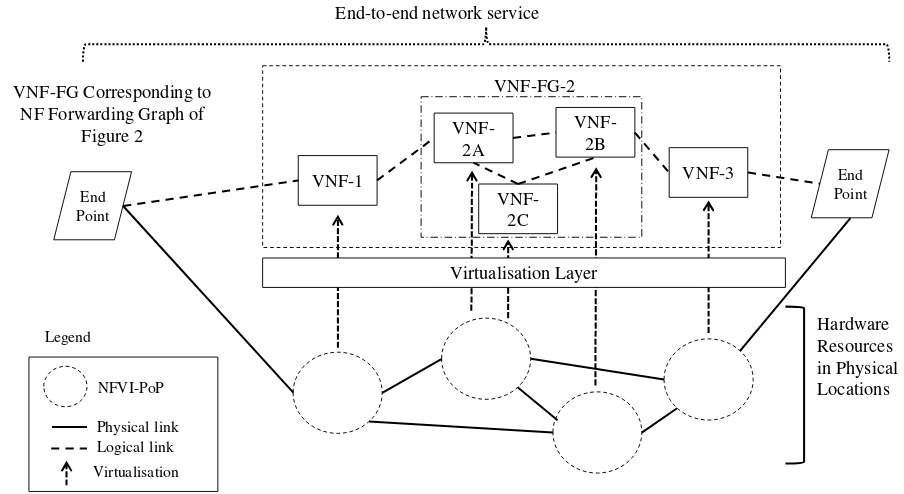
\includegraphics[width=0.49\textwidth]{images/nfv_forwarding.png}
	\caption{NFV forwarding to establish end-to-end connections \cite{ etsi1etsi}}
	\label{img:nfv_forward}
\end{figure}

\subsubsection{Motivating Use Case: EPC Virtualization}
At this point it seems appropriate to present a motivating use case where the previously discussed technologies can be demonstrated and which hopefully serves to highlight the inherent advantages. In 4G networks, one of the components is the so-called Evolved Packet Core or EPC. This part of the network is designed to provide the core network infrastructure and has its origins in GSM from where it was continuously upgraded. The breaking change introduced in 4G was the reliance upon Internet Protocol (IP) as the basic protocol to provide all services. 

\begin{figure}[H]
	\centering
	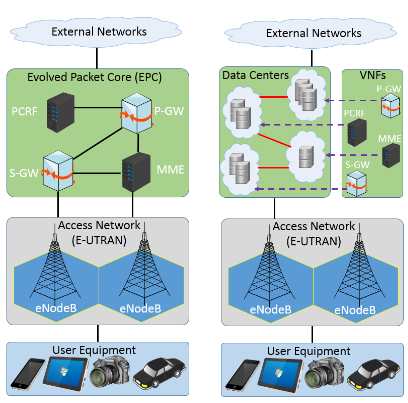
\includegraphics[width=0.5\textwidth]{images/epc_virt.png}
	\caption{Virtualization of the Evolved Packet Core \cite{mijumbi2016network}}
	\label{img:epc_virt}
\end{figure}

Figure \ref{img:epc_virt} on the left side shows how the several components of the EPC are realized with physical middleboxes and puts it into the perspective of a 4G network. . The first component of the EPC is the Policy and Charging Rules Function Server, whose main function is to take care of the service policy and Quality of Service information on a per-user basis. Establishing connection to external networks is the purpose of the Packet Data Network Gateway, connected with the Serving Gateway. The Mobility Management Entity offers control features with regard to the user equipment which is in most cases not stationary and needs to be able to connect and authenticate in a radio network environment. The physical connection of user equipment (bottom) is being established in a 4G network over the eNodeB base stations that use standardized radio frequencies. The scenario to the right shows how this architecture can be realized when dropping expensive, hard to manage vendor-specific black boxes and rather providing the functionality of the components in a virtualized manner. Scaling and replication can be done via multiple deployments of the same VNF on general purpose hardware found in the supporting data centers. The possibilities at this point are manifold, the Infrastructure as a Service (IaaS) cloud service model for instance allows to rent virtual machines in public clouds, which can complement the private cloud capabilities. 

In comparison with the traditional setup, scaling, updating and many other critical operations can now be performed in a much more economical manner. If load spikes hit the system, deploying new VM instances should take care of the incoming, additional traffic. The overall cost sinks, since only the service needed has to be payed, instead of having to purchase additional function specific devices in case of increased demand \cite{4g} \cite{mijumbi2016network}. 


\subsubsection{5G Network Requirements}
As 5G deployment has already started in various locations and can be considered a disruptive technology, its importance in the context of network softwarization shall briefly be explored in the following. In 2017 ETSI published a white paper outlining the most important aspects of NFV in the context of fith generation networks, from the network operators' perspective. The vision of 5G certainly is not limited to ``just'' higher bandwith in the up- /download  direction and lower latency. These advancements are one important element and contribute to a broader vision of  building a true, next generation network that is characterized by ``[\dots] agile resilient converged fixed/mobile networks based on NFV and SDN technologies and capable of supporting network functions and applications encompassing different domains, including serving remote areas and inside buildings'' \cite{nfv5g}. Building on this vision, new and previously unrealistic use cases and business applications can be designed upon the promise of the highly flexible and high-performance characteristics of this new network. In order to realize services complex network services, several technologies need to be taken advantage of. 

%Guaranteeing low latency for instance is a combination of multiple efforts 
First, Network slicing has been identified as a central feature of 5G, heavily relying upon NFVs and other softwarization efforts to be implemented. Network slicing can be understood as the realization of the Network as a service paradigm, where a slice consolidates a subset of the underlying resources in order to provide a custom tailed segment of the network. The components of a slice range from computing, storage and networking resources, often realized with VNFs and for traffic organization SDN and VNF Management and Orchestration elements such as control, management, orchestration and service planes. This service models allows the usage of the network by multiple tenants and each can be shaped by to one's exact needs by varying parameters.
 
Second, and this will be discussed later in more detail, are the Cloud-native Network Functions (CNF).  Virtualization has been the de-facto standard for the definition, deployment and operation of VNFs since their definition. The transformation from PNFs to VNFs has often been simplistic, meaning that the functionality contained in the physical boxes, has just been replicated in a virtual machine. This makes the transition easier, since it is an incremental step, but to further exploit the benefits VNFs can provide, especially in 5G, more agile and lightweight approaches have to be explored. 

Third stands the end-to-end service management that is closely related to network slicing. A new technology claims high investment to setup and is only justified if there is a realistic promise of new business prospects and models. Providing custom network services that are located between the two end points of communication as a service is essential to 5G networks. This simple sounding principle is extremely complex in an operational and management sense. When customers compile their own service from available components, these elements need to be reserved, provisioned, monitored and billed. Providing means to manage these services is a significant effort, that needs to take into consideration many aspects like lifecycle management, monitoring and debugging and many more, always increasing the complexity. 

Lastly, the laws of nature prohibit that for certain scenarios with strict latency requirements, the length of the service function chain exceeds a specific distance. If an application, for instance augmented or vitual reality or tactile internet like remote surgery, are being designed, they will postulate strict latency requirements that will require a round trip time of under 2ms. Light travels approximately 300km in 1ms, excluding refraction and reflection.  This severely limits the radius a network service can effectively be used. Since not all functions are required for a specific use case, splitting them up and allowing for a highly distributed placement along the lines of microservices might solve this problem. In reality, this can be realized with smaller, but numerous data centers that are closer to the users, thus lowering the distances needed to travel. This is known as edge computing in general or fog computing as defined by Cisco \cite{ordonez2017network} \cite{nfv5g} \cite{alexgalis2018multi} \cite{alexgalis2017analysis} \cite{cn5gvnf} \cite{de2019network}. 


All in all the growing capabilities of the fifth generation network can only be efficiently made use of and marketed, if the infrastructure is flexible enough to allow for all of this. 

% NFV to microservices and containerization???

\subsubsection{NFV Issues}
% Problems? Copy 1:1 hw appliance to vm, not efficient, throughput/all traffic guided through commodity hardware (-> dpdk) ; Added complexity! Placing functions? No autohealing, scaling, load-balancing, etc. Resilience? Fault-tolerance? Public vs Private cloud




\cite{nfv_wp} \cite{nfv_etsi}

\begin{comment}
	
\begin{figure}[H]
	\centering
	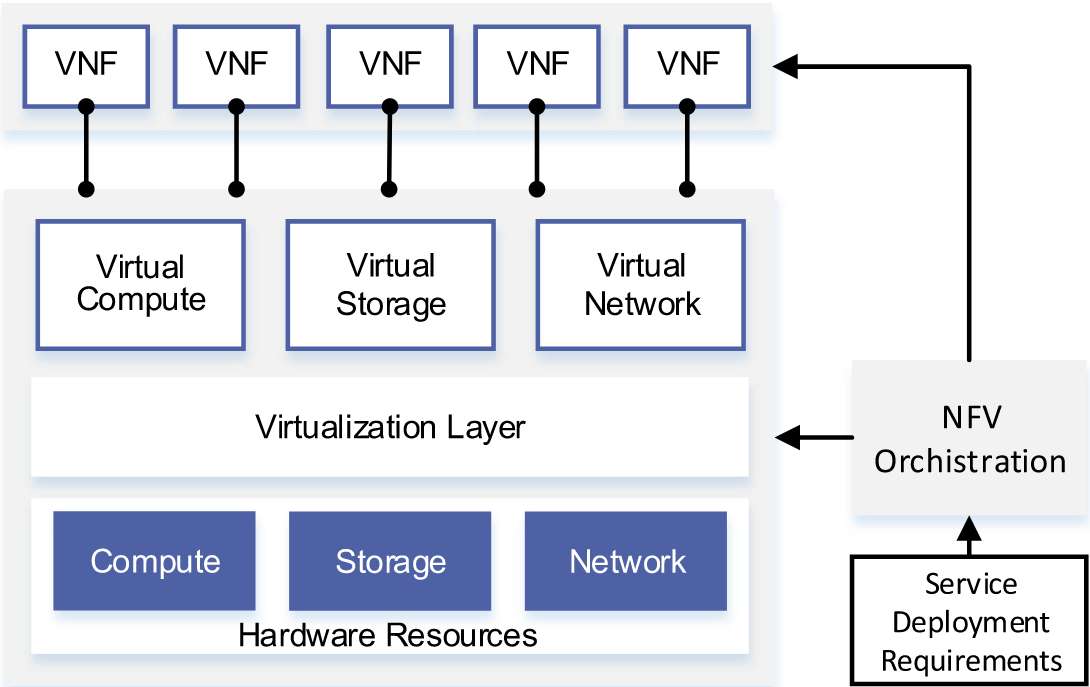
\includegraphics[width=1\linewidth]{images/nfvi.png}
	\caption{Schematic network architecture using virtual network functions \cite{li2015software}}
	\label{img:nfvi}
\end{figure}

\end{comment}




\section{Cloud-native NFV}
Network virtualization and especially the switch from network functions residing inside purpose specific hardware towards VNFs, have been introduced in section \ref{sec:networkV}. The advantages are manifold, and include but are not limited to the following: Reduce the physical complexity of networks by eliminating the need for a majority of function-specific black boxes. This also causes a decline in setup and operational costs, since the highly specialized devices are expensive, consume more power and also require significant personel hours. This is mainly due to their vendor-specific functionality, and the need to physically install and configure them with limited possibilities of automation. Building new network services has become much easier and faster and can result in faster time to market while also ensuring higher return of investment. Reacting to fluctuating has become much easier and cost efficient. Finally, since the functionality is only bundled in software the emergence of ecosystems provide a more competitive market and favors innovative ideas. 

\subsection{NFV shortcomings}
This is definitely a step into the right direction towards a leaner and future proof network design. VNFs have been essential to redesigning networks and allowing for new use cases and business models. As much as this is a breakthrough, there are still some shortcomings of this approach that need to be considered. 

As previously explained, the main virtualization technique in VNFs has mainly been the virtual machine. Initially, the focus was on porting the functionality from a physical box into a virtual software artifact that runs inside a VM. The resulting functions are equally vertically integrated as their original, physical counterparts, following a rather monolithic approach. This has two main drawbacks:
First, the hypervisor-based virtualization is generally considered very resource heavy, due to inherent redundancy. On top of the host's infrastructure and operating system, a hypervisor orchestrates the the resource access of the guest's operating system (OS). Each instance of a VM on the same host has to rely on the hypervisor to get access to the resources that its OS can then use. 
Second, it is not enough to just port the VNF to use a container instead, the payoff would be minimal. Instead, the problem lies in the monolithic architecture of the function, which prevents a more flexible approach to service composition. Splitting up highly complex functions into logically separated, small and stateless components has multiple benefits, among which are more efficient resource utilization with much more appropriate scaling. Additionally, this allows for a more fine grained service composition and facilitating the development effort immensely by allowing for easier automation efforts. 

% NFV to microservices and containerization???
% Problems? Copy 1:1 hw appliance to vm, not efficient, throughput/all traffic guided through commodity hardware (-> dpdk) ; Added complexity! Placing functions? No autohealing, scaling, load-balancing, etc. Resilience? Fault-tolerance? Public vs Private cloud
%NFV and VNF basics \cite{mijumbi2016network} NFV real-world impact \cite{bilal2016impact} Service orchestration \cite{de2019network}


\subsection{Enabling Technologies and Concepts}
Mitigating the shortcomings of traditional VNFs can be realized by using specific technologies and adhering to cloud-native development principals. Such enabling technologies will be explored in the following.

\subsubsection{Docker}
Opposing the the concept of hypervisor-based virtualization is that of container-based virtualization which eliminates the need for a dedicated version of an OS with all its stack in each VM instance. It rather makes use of the host's kernel directly, circumventing a lot of the overhead a VM introduces. Figure \ref{fig:docker} shows the two approaches in contrast to each other. The most famous container project is called Docker. 

\begin{figure}[h]%
	\centering
	\subfloat[Hypervisor-based virtualization]{{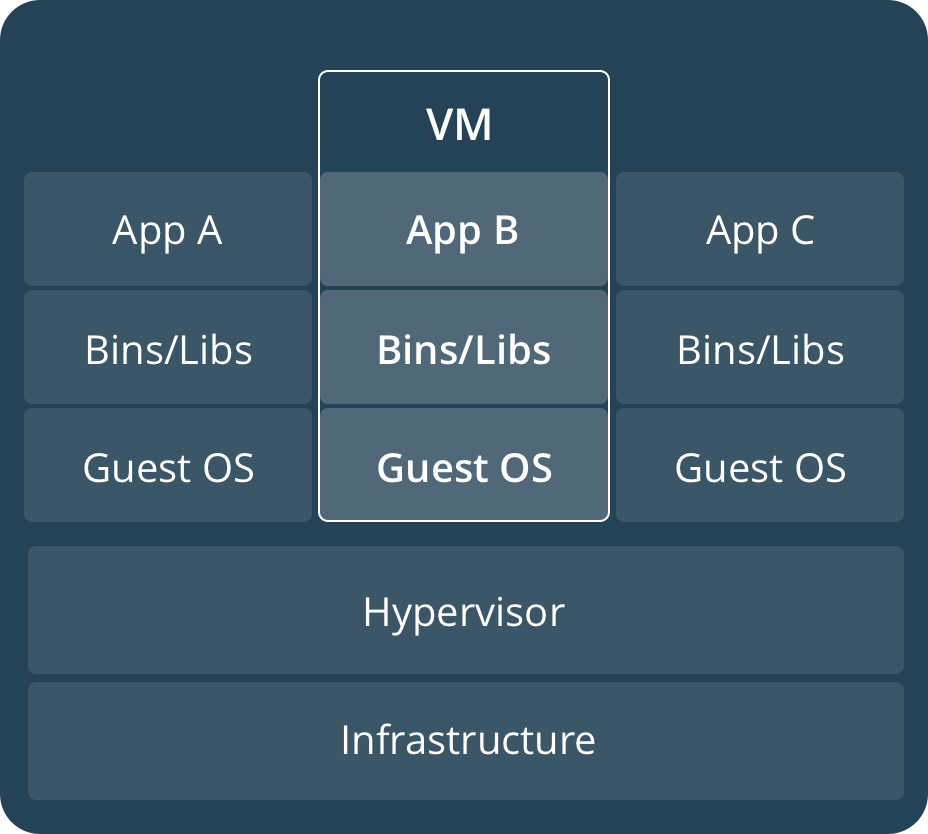
\includegraphics[width=.45\linewidth]{images/vm.png} }}%
	\quad
	\subfloat[Docker container]{{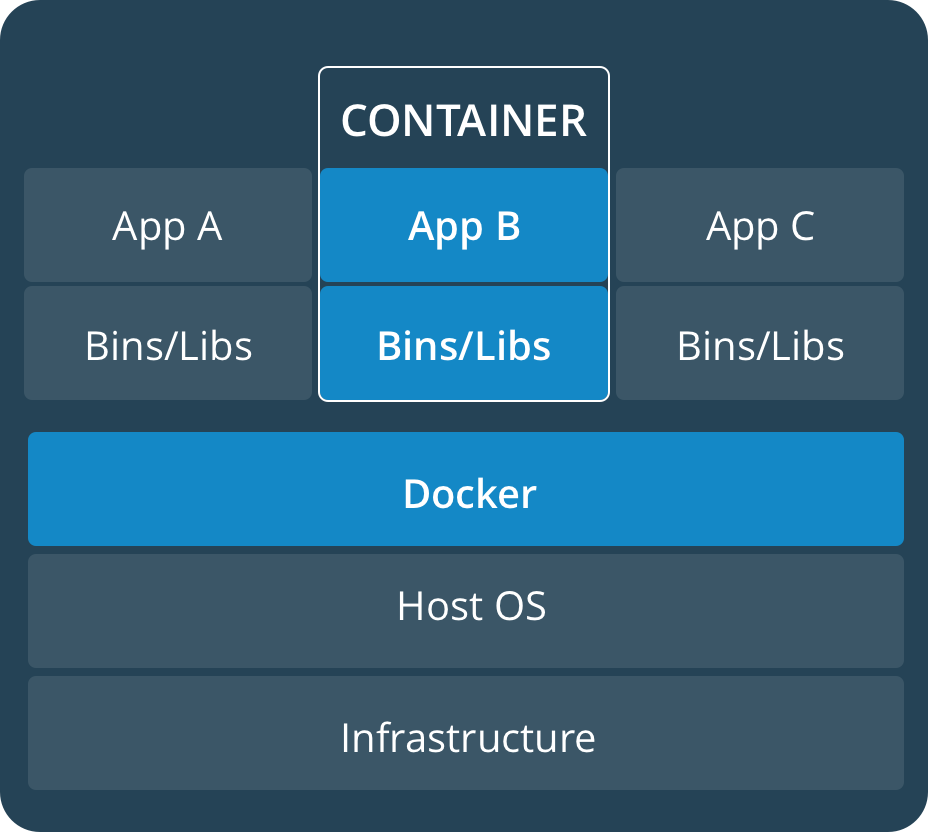
\includegraphics[width=.45\linewidth]{images/dockerContainer.png} }}%
	
	\caption{Comparison between hypervisor-based virtualization and Docker \cite{dockerdocu}}
	\label{fig:docker}
\end{figure}

It is an open source project that was originally build from many preexisting technologies in order to provide a more efficient virtualization technique as opposed to VMs. The tools that were used are mostly part of the Linux kernel as for example control groups (cgroups), used to manage and orchestrate the resource usage of a group of processes. Together with namespaces , that provide means to make resources only visible to a set of processes, they build the basis to separate the executable units from each other. These units are called \textit{containers} and are executed by the docker host via the system's kernel, using features like cgroups, namespaces, linux security models and many others to ensure strict separation from the rest of the system. Defining the composition and behavior of such a container is being done with so-called images. They are the blueprint, from which multiple containers can be derived from encapsulating the predefined contents inside multiple, read-only filesystem layers. Containers have a thin, writable layer at their disposal which is ephemeral. For persistence, volumes can be used to share data between the host and the container environment. The layering system in docker strives to minimize redundancies by sharing identical layers between multiple images, keeping the overall storage needs low \cite{fink2014docker} \cite{morabito2015hypervisors}.

Docker has gained a lot of popoularity over recent years and as an open source project, it has favored the creation of a large ecosystem around it. This makes the usage of docker much easier, since documentation, community help and tutorials are readily available. When packaging an application or a service inside an image, often dependencies and libraries need to be included. The large ecosystem makes this almost painless, since many, official and verified images already exist that can be used as a basis.

\subsubsection{OVS and OpenFlow}
Provisioning network functionality inside containers necessitates that the attachment of the containers to the rest of the network can be realized with as much automation as possible, and secondly with high performance. Attaching the containers to virtual switches is an essential step since these can guarantee both of these requirements. 

Open vSwitch is such a switch, using the Openflow protocol to be able to communicate with an SDN controller and thus provide programmability. Since Linux Kernel 3.3, it it comes bundled in it and provides multi layer switches and additional tools for a consistent setup, configuration and monitoring. The documentation provides insight into the authors' vision of what its main purpose is: Making networking easier in multi-server deployments that heavily rely on virtualization. In support of this high-reaching goal are several design characteristics: Making the migration of entities in the network as easy as possible is one of the core advantages of VNFs and CNFs and is realized by allowing the migration of configuration with the associated host. Supporting automation of the network is the fact that OVS holds the state in a database (OVSDB) while supporting triggering events remotely. OVS supports the idea of separating network traffic logically by tagging the packets. Finally, high performance during the interplay of hard- and software is guaranteed by allowing the forwarding path of the bridges to use the in-kernel datapath and directly communicating with the network interface cards (NIC). This also allows for simultaneous management of physical and software networking entities with teh same technology. 

Figure \ref{img:ovs} shows how the different components of OVS interact. The OVSDB is located at the user space level and stores all the information about the virtual switch. Its contents is accessible via the SDN controller in the network, or the ovs-server.
Realizing the actual switch is the ovs-vswitchd daemon, located in user space. Communication and manipulation is being realized via the OpenFlow protocol and the Southbound API of the SDN controller. 
\cite{openvswitch} \cite{pfaff2015design}. 

\begin{figure}[h]
	\centering
	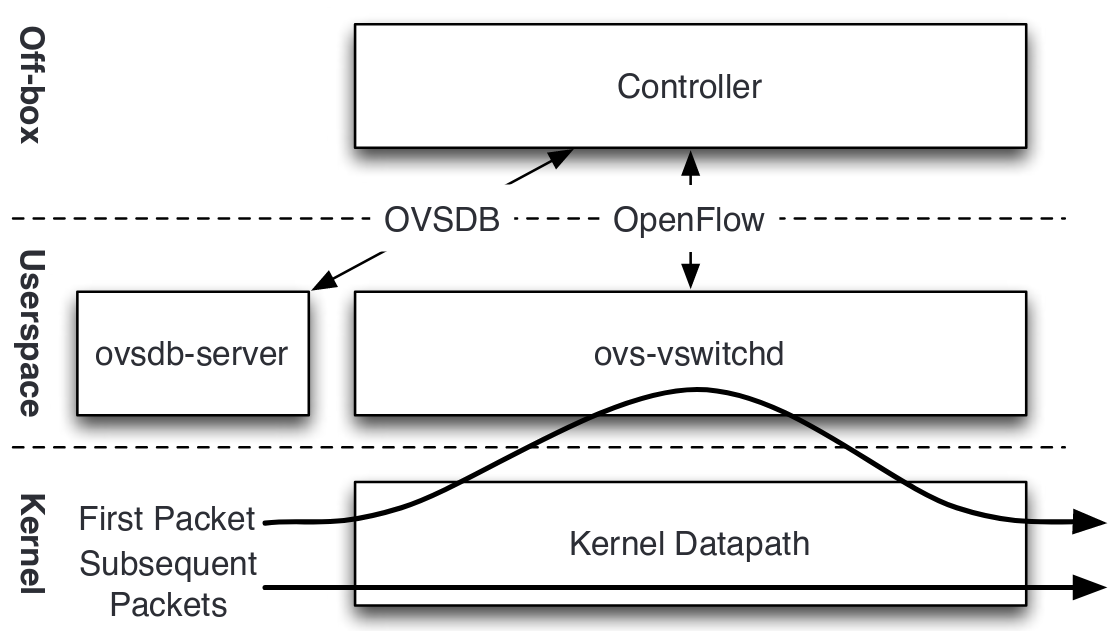
\includegraphics[width=1\linewidth]{images/openvswitch.png}
	\caption{Components and interfaces of Open vSwitch, source \cite{pfaff2015design}}
	\label{img:ovs}
\end{figure}

The OpenFlow protocol was developed in an educational environment by McKeown \textit{et al.} \cite{mckeown2008openflow} in 2008. Its main focus was to allow researchers to conduct experiments in their networks, while being "[...] open, vendor neutral, control-data plane interface [...]" \cite{berde2014onos}. Realizing its potential, the Open Networking Foundation (ONF) has adopted management and supports the extension and further development of OpenFlow.
In traditional forwarding switches packets are being registered from the ports they arrive, analyzed, and from the information in the packets' header specific rules for how to deal with them are learned. The inner workings of this behavior are transparent to the user without a possibility to modify or extend. In contrast, OpenFlow provides a possibility to manipulate so-called flow tables, that represent the rules of how to deal with incoming packets. 
Figure \ref{img:of} shows such a flow table that prescribes what to do with incoming packets as prescribed by the SDN controller. For each packet, a rule will be looked up from top to bottom which will prescribe the behavior exactly.  Information that can be used to match are various, like for example the MAC and IP addresses, port information and many others. In the figure these fields are marked in white color. The first column in grey prescribes what to do with a certain packet. For instance if a packet is destined to TCP port 25, it shall be dropped. Wildcards can be used and if nothing matches, the last line says to send the packet to the controller. Finally, the last column shows another advantage: Metrics for analysis of how often a rule has been applied. 
\cite{mckeown2008openflow}. 

\begin{figure}[h]
	\centering
	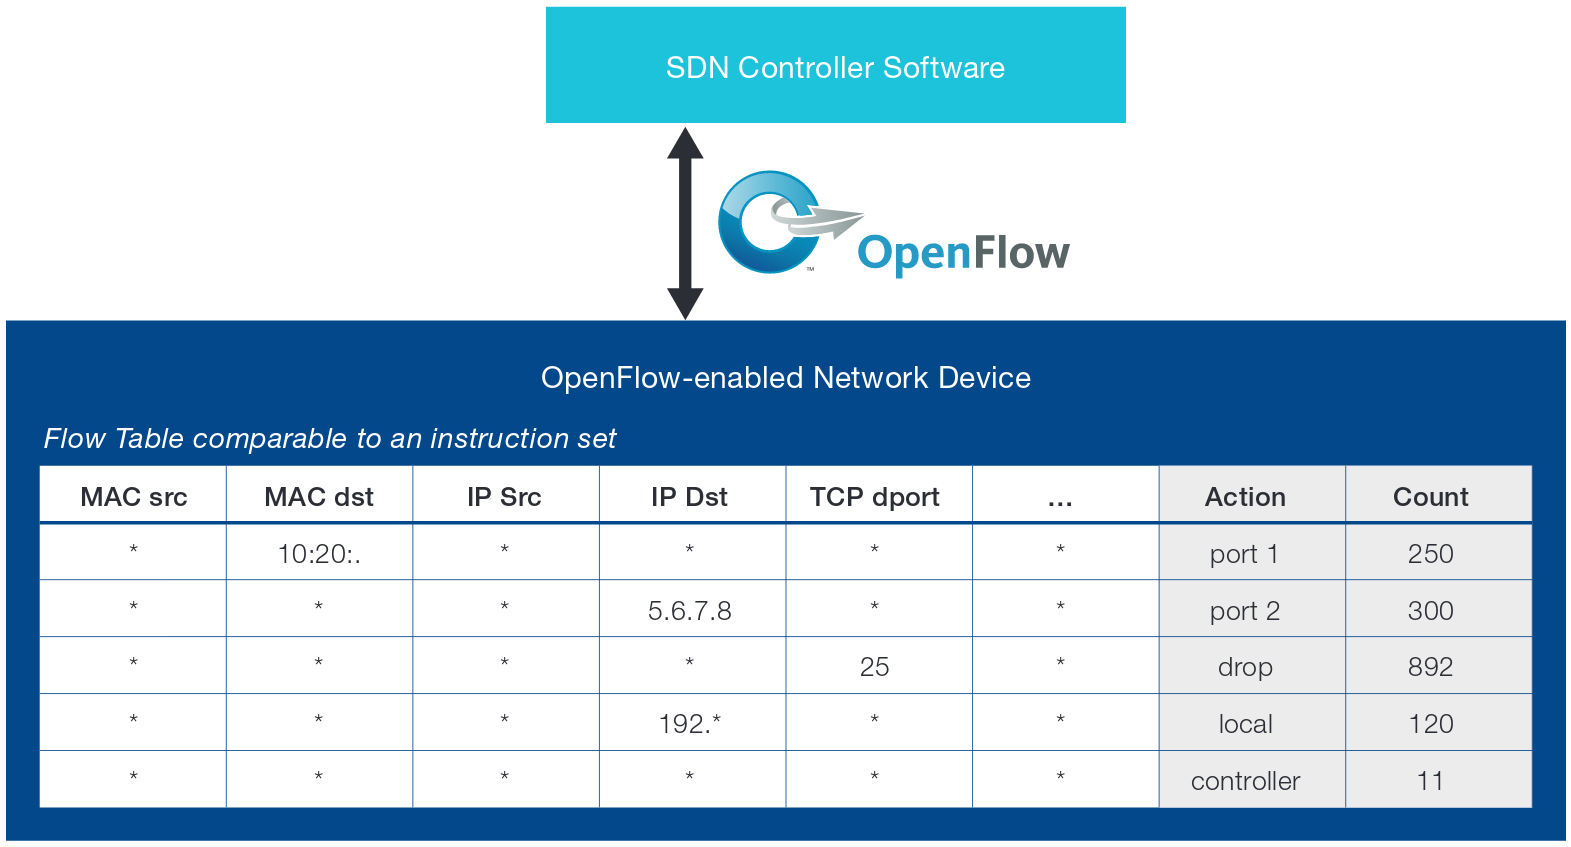
\includegraphics[width=1\linewidth]{images/of.png}
	\caption{Example of OpenFlow Instruction Set, source \cite{ofWhitePaper}}
	\label{img:of}
\end{figure}

This matching information can be manifold and includes but is not limited to the MAC/IP addresses of the sender or the receiver, the incoming port etc. In Figure \ref{img:of} these fields can be found on the left and are marked in white color. The two fields on the right serve a different purpose. The entry in the \textit{Action} column specifies what needs to be done to the packet if it conforms to the specified criteria. In this example it will either be output via port 1 or 2, dropped if it is directed at a TCP destination port 25, sent to local for processing if the IP destination starts with 192 or sent to the controller if no other rule applies. 

\subsubsection{Kubernetes}

All in all, the combination of these technologies renders unforeseen automation possible, especially in the network domain. When deploying functionality bundled in Docker containers however, interacting directly with the Docker hosts on each compute node for each deployment is very cumbersome. There is the need for a system that manages multiple hosts, provides lifecycle management, load-balancing and scaling. 

Kubernetes is such a system that was developed by Google for its internal needs. The motivation was the handling and usage of Linux containers and the need arose for a management system. Since non existed, the company started developing its own. After building Borg and Omega as closed source systems, Kubernetes is an open source project and can be used in different environments, best known is Google's own public cloud service. 

\begin{figure}[h]
	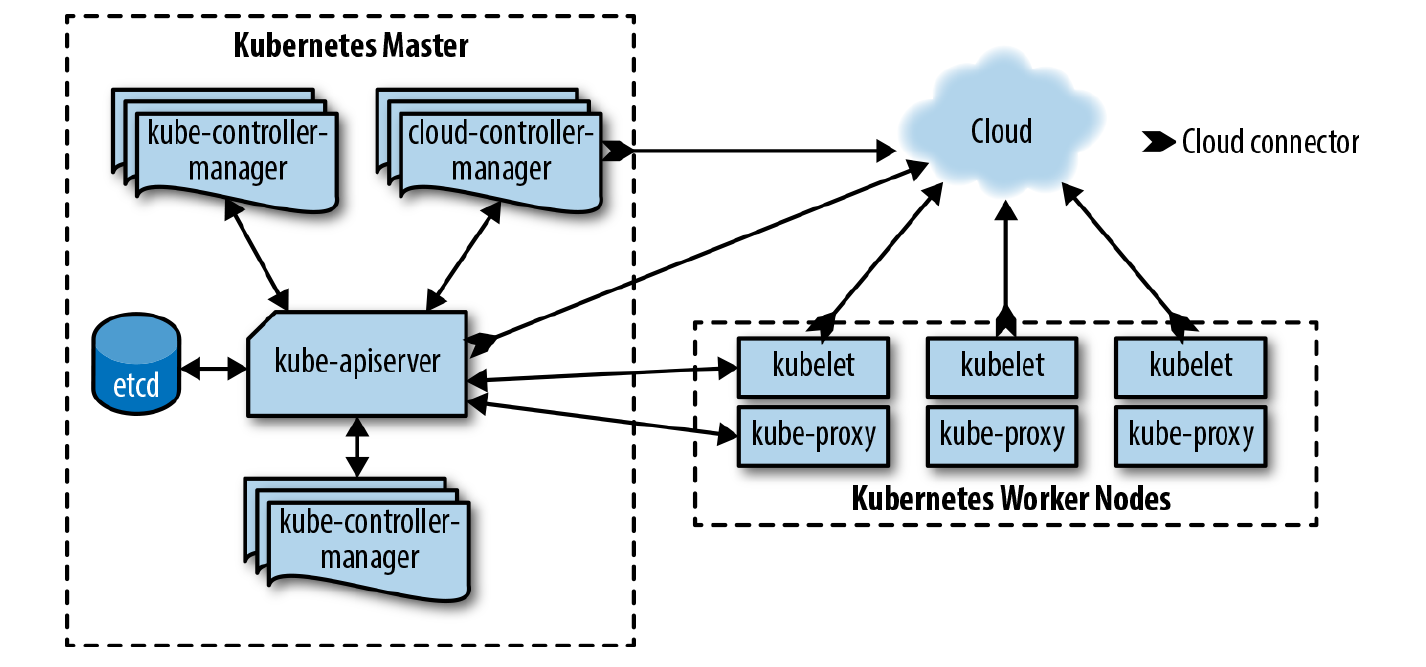
\includegraphics[width=\linewidth]{images/k8Arch.png}
	\caption{Kubernetes Components and their relationship \cite{k8CN}}
	\label{fig:k8}
\end{figure}

Figure \ref{fig:k8} summarizes briefly the components of the orchestration system that manages a cluster. One Master manages multiple worker nodes, and generally speaking is not available for application-specific workloads. The single processes doing the orchestration are the following:

\setlength{\leftmargini}{0pt} 
\begin{description}
	\item [kube-controller-manager] A daemon, managing several different controllers who know the desired state of the cluster and try to converge the real, observed state towards it. Each controller serves a different domain and has a defined set of responsibilities. Examples are the replication, endpoints, namespace and serviceaccounts controller.
	
	\item [kube-scheduler] This process manages the deployment of defined pods that bundle the execution of one or more containers to worker nodes inside the cluster. In order to make a sensible selection, the scheduler needs to know the resource usage of the worker nodes. Additional constraints that might be specified by the user have to be taken into account, too at this point. This is not explicetly included in fiugre \ref{fig:k8} but an essential part of the control plane.
	
	\item [kube-apiserver] Central to the management of such a highly distributed system is the communication, which is served via JSON over HTTP. Validation and serving of API requests are the scope of work of this component. 
	
\end{description}

Apart from these processes, the manager needs to save the state of the cluster with all relevant information. This is being done in etcd and accessed by the kube-apiserver. The work for controlling the cluster is typically spread over multiple master-nodes to increase fault tolerance and ensure high availability. The etcd database containing the state of all the nodes and the deployments is also replicated and can survive individual failures in the control plane. 

The worker nodes in the cluster are there to provide an environment to execute application specific units. Therefore, a container runtime needs to be provided to start, monitor and stop containers. The process that provides this functionality on the worker nodes is called a kubelet. Ensuring communication not only within the cluster, but also with the rest of the attached network is the kube-proxy. When a worker node failes, the control plane will react to this event and try to mitigate the impact on the overall deployment automatically and ensure availability. Diverting the workload to other worker nodes naturally only works as long as resources are still available in the cluster. 

To sum up, Kubernetes provides a comprehensive management and orchestration framework for containerized applications. A unified approach to orchestrate, manage the lifecycle and monitor the status facilitates the cloud deployment. The general layout of the system is highly distributed and allows the usage of an overlay-network using Open vSwitch. This ensures that high networking performance and flexibility that is needed when building carrier-grade network functions. Additionally, the switches can be managed remotely via an SDN controller. \cite{burns2016borg} \cite{kubernetesUp} \cite{k8CN}


\subsubsection{Cloud-native paradigm}
%OVS switches, SDN and Openflow allow for unprecedented possibilities to automate network setup and orchestration. This  
Software engineering practices have moved in recent years from monolithic approaches towards a microservice architecture. The main characteristic and motivation behind this shift is manifold: Making software more compartmentalized ensures a loose coupling that allows for easier development and upkeep of complex applications. These advantages prescribe the adherence to certain design principles to fully exploit them. 
Developers at Heroku, especially Adam Wiggins, have summarized these principles into the twelve factor methodology that takes into account the distributed environment of the cloud. Their methodology cloud provider agnostic and helps guide developers towards building software on such a high level of abstraction where automation is key. The 12 factors are as follows:

\setlength{\leftmargini}{0pt} 
\begin{description}
	\item[Codebase] When developing an application, it is paramount to avoid fragmentation and keep everything in revision control (e.g. GIT). From one codebase, all the deploys, such as testing or production environments should be started. This ensures reproducibility and reduces the complexity. If multiple repositories with different codebases exist, each can be twelve factor app compliant and together they would form a distributed system.
	\item[Dependencies] An automated approach that creates an executable software fragment needs to have explicit access to all dependencies needed and thus developers have to declare them. This ensures unproblematic deployment in the target environment since assumptions about the existence of dependencies in the environment are forbidden. 
	\item[Config] Since there is only one codebase, but multiple deploys on possibly heterogeneous systems, manipulating certain behavior is necessary. This has to be solved by storing configuration in the respective environment. Often configuration variables are stored in constants, which does not allow to make adjustments without the need for rebuilding the complete application. This can be avoided by considering a deployment as bringing together a build artifact and configuration on an execution environment.
	\item[Backing Services] All related services that are being used need to be treated as resources and thus be detachable and attachable. This allows swapping out services like database for instance without having to adapt the code. 
	\item[Build, release, run] For each stage, build, release and run, a strict separation needs to be ensured as to not introduce unforeseen behavior. Running a load test against the production environment could be detrimental to the user experience for instance. 
	\item[Processes] The application shall be realized as a set of stateless processes ensuring proper loose coupling and no side effects. Persistence should be organized with attached resources/services, for instance a remote database. For caching purposes however, using the local file system is acceptable. When a cloud function for instances needs to process a large image in multiple steps, it can use the local filesystem. The results need to be persisted appropriately to not be lost.
	\item[Port Binding] Inter-service communication is very important and should be realized via listening on exposed ports. The underlying thought is making the twelve factor app completely self-contained. By relying on port-based communication, each app can become the backing service of another by declaring its URL in the configuration of possible consumers. 
	\item[Concurrency] Since the application should be built as an accumulation of stateless processes, scaling can be realized by replicating the needed process.
	\item[Disposability] The single processes have to be disposable. Additionally, setup and teardown should be quick to realize to ensure robustness. 
	\item[Dev/prod parity] Developing in an environment that is as close to the actual production environment as possible ensures easier deployments.
	\item[Logs] Logging is essential to debug an application and monitor it during execution. All processes treat logs as event streams and use \textit{stdout} and \textit{stderr} to facilitate aggregation by the execution environment. 
	\item[Admin processes] Tasks of administrative nature (e.g. database migration) should be executed as one-off tasks and kept close the application sources to ensure reproducibility.
\end{description}

When an application is developed from the ground up with this methodology in mind, it can be called cloud-native. It should be clear by now that simply deploying a monolithic, classical application inside a VM or a single container is possible, but not appropriate for the cloud environment since its advantages can not be fully exploited \cite{hofmann2017microservices} \cite{12Factor}.

\begin{comment}
	
\begin{figure}[h]
	\centering
	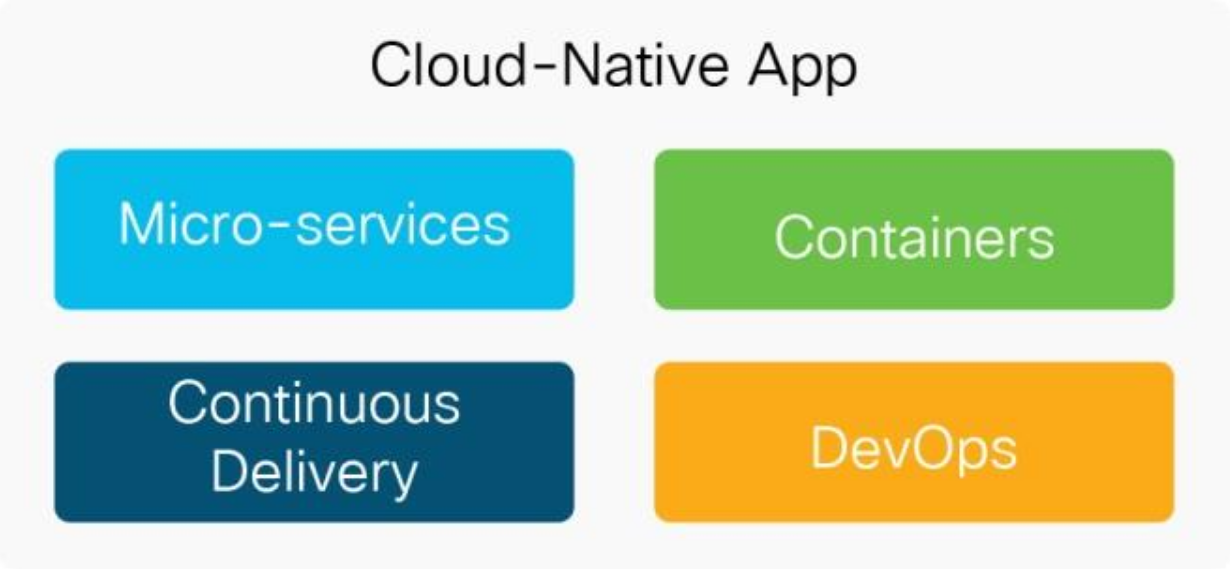
\includegraphics[width=0.75\linewidth]{images/cloudNativeApp.png}
	\caption{The principals of a cloud-native application as defined by the CNF \cite{CNF}}
	\label{img:cloudNativeApp}
\end{figure}
\end{comment}



\subsection{CNFs}
Powerful concepts have been introduced that can be used for different purposes when designing a network function that should conform to the cloud native paradigm: Containerization as an alternative concept to more heavyweight, hypervisor based virtualization. Orchestration and management of containerized services can be accomplished by Kubernetes that takes care of multiple issues: Deployment, lifecycle management, fault-tolerance, scaling and load-balancing. The Network Function Virtualization Infrastructure, responsible for providing an environment to deploy VNFs to, can for instance be realized by using Kubernetes internally. Making use of the clustering concept ensures that the abstraction from multiple, physical compute nodes can happen seamlessly while ensuring their efficient usage. Management and monitoring functionality is well documented and built in, reducing the complexity of the Virtualized Infrastructure Managers. Their role shifts towards managing and monitoring the Kubernetes clusters available. Ensuring dynamic and flexible interconnection of the different components on the physical, as well as the virtual level can be accomplished with SDN and the switches under its domain. Open vSwitches and OpenFlow provide an easy and high performance way of interconnecting the different components dynamically. 

Realizing this vision is in the scope of Cloud-native Network Functions. When NFV was proposed by ETSI in 2012 in a white paper, work on Docker and Kubernetes had not started yet. The status quo were a plethora of physical middleboxes providing specialized functionality and the cloud had not the importance it holds today. Even so, cloud-native principles can be recognized in identified challenges of the document. Portability between several hardware vendors and different virtualization realization (e.g. hypervisors) had been identified. Management and Orchestration and automation efforts are central to scalability and profitable operations. The idea of building systems that can tolerate partial failures and are robust is still important to cloud native application development.
In the 2017 revision of the white paper, ETSI explicitly picked up the CNF concept. The additional benefit, especially in delimitation to VNFs is the fact that the functions are designed from the ground up with the execution in a cloud environment in mind. 

The acceptance of this new paradigm is steadily rising, various vendors and initiative explore its possible usage scenarios and propose ways of adapting it on various abstraction levels (i.e. from high level architectures to actual products). 
The 5G-PPP (5G Infrastructure Public Private Partnership) initiative for instance has released a white paper titled \textit{From Webscale to Telco, the Cloud Native Journey} \cite{5gppp} that specifically tries to apply the experiences and best practices gathered in the cloud application engineering to the networking domain. The self-proclaimed goa is to ``[\dots] avoid the risk that 5G remains a niche connectivity gap-filler largely ignored by cloud applications and services boom'' \cite{5gppp}. The risk stems from the fact that this technology is very expensive, and can only become profitable when the new possibilities are fully taken advantage of. This entails providing end-to-end services on a per-customer basis, which poses considerable challenges. These can only be achieved, when fully embracing all the previously mentioned concepts and taking them into consideration when designing both, the Virtualized Network Functions, as well as the infrastructure they are supposed to be deployed to \cite{5gppp}.




% Implementations NFV4ARM
\begin{figure}[h]
	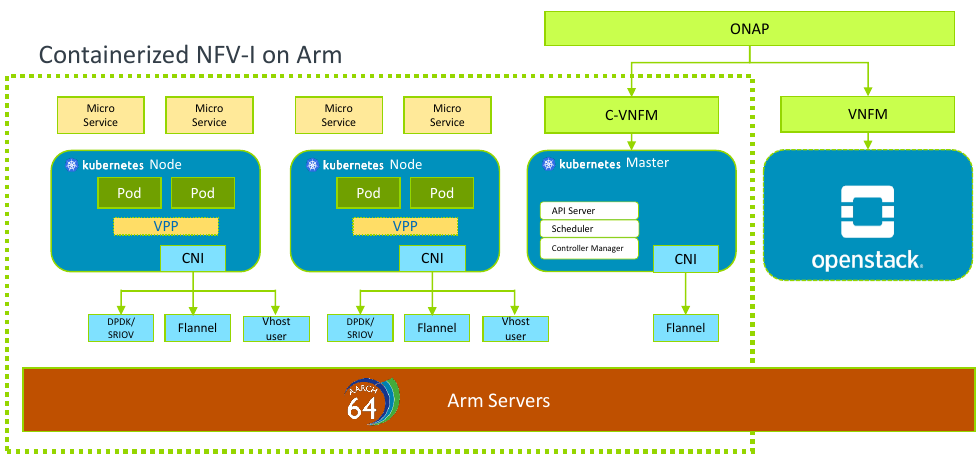
\includegraphics[width=\linewidth]{images/nfv4arm.png}
	\caption{ONAP extension for NFV on ARM \cite{nfv4arm}}
	\label{fig:nfv4arm}
\end{figure}

Implementing the Cloud-native Network Function (CNF) functionality in orchestrator software already exists and can serve to showcase how this can be realized. An extension to the Open Network Automation Platform (ONAP), part of the Linux Foundation that exposes a southbound API to communicate with a NFVI/VIM, can be seen in figure \ref{fig:nfv4arm}. This is a hybrid model since over the southbound API a classical VNF Manager (VNFM) is attached that uses openstack to manage virtual machines and additionally, a Containerized-VNFM has been registered to the automation platform. This manager coordinates the CNF deployment via directly via the kubernetes master node, that is in charge of the different worker nodes. 


\begin{comment}
	“Lift and shift” architectures brought certain benefits of virtualization, mostly related to the fact that
	the hardware can be shared between different functions. However, they did not solve issues related to scaling, feature velocity and availability because the code was still a monolith captured in a VM.
	Cloud native (which encompasses the three disciplines mentioned above) is a re-design of the
	network functions themselves.
	Current cloud native systems are focused on managing enterprise and web commerce, not packet
	forwarding. The purpose of this paper is to show that all the issues related to building a cloud native
	NFVs are solvable problems. The design principals that made cloud native a success can be applied
	to network function virtualization as well, driving the same service velocity, availability and scaling
	to the networking world.
	
	cloud native network function virtualization true cloud for nfv
\end{comment}



\begin{comment}

\begin{figure}[h]
	\centering
	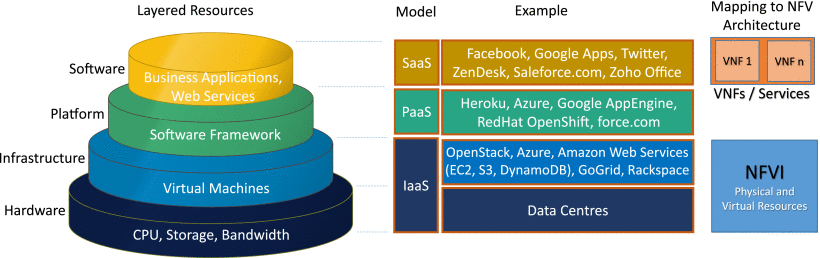
\includegraphics[width=1\linewidth]{images/arch.png}
	\caption{This is the caption \cite{mijumbi2016network}}
	\label{img:arch}
\end{figure}

\end{comment}

\section{Enabling Technologies}
Extending Networking into the Virtualization Layer (see \cite{pfaff2009extending}) summarizes how the traditionally monolithic and physically bound domain of networking can be broken up and modularized by means of virtualization. The following three parts would focus on enabling and supporting technologies needed to realize the vision of this new paradigm. First, the business logic needs to be packaged and executed. This can happen in virtual machines, containers etc. Following that, virtualized switching technology needs to be put in place to allow for successful packet forwarding. One technology is Open vSwitch which is an implementation of a virtual switch, connecting virtual interfaces of VMs for instance with physical interfaces. Docker and Kubernetes additionally provide means for communication between several, executable artifacts.


\quad




%\begin{description}
%	\item [VNF] Can complement the SDN paradigm (but can exist independently)  by providing functionality needed in the network domain as an executable artifact
%	\item [NFV] NFV integrates VNFs into a system that can manage and deploy these functions in sensible manner. 
%\end{description}

%\subsubsection{Organizations and Motivations}
%ETSI proposing NFV architecture already in 2012 in a white paper  \cite{nfv_wp}. The CNCF (Cloud-native Computing Foundation) has launched a testbed to compare the performance of VNFs on an OpenStack enviromnent versus a Kubernetes setup \footnote{https://www.cncf.io/announcement/2019/02/25/cncf-launches-cloud-native-network-functions-cnf-testbed/}	



\section{Conclusion}

\subsection{Summary}
In this paper, the basic concepts of how functions are being developed, deployed and managed in large scale networks have been explored.An overview and evaluation of concepts that have been put forward to tackle the limitations of traditional networks by applying the cloud native principles to the network domain has been given.
Since this domain is very specific to the Internet Service and Telecommunications providers, special requirements okay a crucial role like reliability and high performance. The reliability aspect has contributed to the fact that there is a certain hesitation to switch from proven, old concepts to more modern and flexible solutions. This can be exemplified with packaging functionalities inside physical boxes, to virtually abstracting from general purpose hardware and bundling the functionality in software artifacts. NFV was proposed in 2012 and the concept of using virtual machines, organized via Open Stack has since been implemented in many networks. The recent advancements of the public (and private) cloud providers in providing progressively cheaper and remote service models has caused a paradigm shift in software architecture and engineering. Using advancements like microservices, design considerations like from the 12-factor app and CI/CD pipelines and softwarized network technologies like SDN to further automation, lays the foundation for more intricate business cases for fifth generation networks.

\subsection{Future Work}
%Future Work typically means what YOU would do if you had infinite time for your research. Not what the technology will be in the future. Try to use a different name for that section. Or did I read that wrongly?
The field of Cloud-native Network Functions is just starting to get to the point where first, interesting results can be observed. Often these are limited to proofs-of-concept and calls to action, but other projects have started implementing NFV-Infrastructures which have not yet been exhaustively researched. Additionally, the technical limitations of Kubernetes and Docker in the domain of the telco domain have not been touched upon in this paper, since it serves as an introduction to this complex subject. An interesting field of investigation would be the specific interconnection of the containers and pods and how application traffic can be guaranteed to flow with high performance. As an outlook, DPDK (Data Plane Development Kit) an open sourced software project developed by Intel has found wide usage in accelerating application packet processing. 

\begin{comment}
	

\section{List of references}
\begin{description}[style=sameline, leftmargin=1em, font=\normalfont]
	\item[Pfaff \cite{pfaff2009extending}]  Virtualization in Networking. Basics of how virtualization started to make its way into the networking domain. Overview of network architectures and topologies that employ virtualization. The starting of how to break up monoplithic network infrastructure with virtualization. The components decsribed here are the basis for VNFs (and the overarching NFV). 
	
	\item[Sherry \cite{sherry2016middleboxes}] Middleboxes as a Cloud Service. Traditional Network Functions are provided by specialized and proprietary middleboxes. What is their significance in 2016's enterprise and educational networks? The results of this paper motivate towards decoupling functionality from physical boxes and providing virtualized solutions.
	
	\item [Mijumbi \cite{mijumbi2016network}] NFV State of the art . Comprehensive overview of the state of the art of NFVs with focus on Telephony Service Providers. Interesting because critical evaluation of NFV solutions that, contrary to their original design, seem to result in a means to pool vendor specific resources together instead of supporting real interoperability. 
	
	\item [Bilal \cite{bilal2016impact}] Impact of CNFs . The authors analyze resource consumption of a real-life example, namely two different mobile networks and evaluate the impact virtualization would have on these networks. 
	
	\item [De Sousa \cite{de2019network}] Network Service Orchestration. The Network Service Orchestration is in the focus of this paper. The authors lay out a comprehensive survey over service orchestration technologies and additionally provide a taxonomy.  
	
	\item[NFV White Paper \cite{nfv_wp}]  The white paper lays out the foundation for NFV. 
	
	\item [AM White Paper \cite{evolutionnfv}] This white paper, seemingly sponsored by  Huawei, focuses on CNFs for telecommunication companies, including migration strategies from NFV to CNFs. 
	
	\item [CNF White Paper by Cisco \cite{CNF}] A white paper sponsored by Cisco provides insights into the point-of-view of a vendor. They set out to define what CNFs are, and how potential clients can benefit from them. They use Kubernetes as the main orchestrator and suggest it for further roles, too. 
	
	\item [Cloud-native 5G \cite{inproceedings}] The authors layout the implementation of VNFs that adhere to Cloud-native design principles for 5G. Furthermore they summarize existing projects and show an exemplary Use Case for this technology. Very relevant to my work, they use Docker for prototyping and are migrating to Kubernetes for the Cloud Native NFVI (Network Functions Virtualization Infrastructure) interface. A NFVI is specified here \cite{mijumbi2016network}.
	
	\todo{5G would also bring in an interesting perspective. You could show what kind of challenges are introduced with 5G for the network as well. }
	\todo{Reference/Specification for NFVI}
	
\end{description}

\end{comment}
